% 
% ======================================================================
\RequirePackage{docswitch}
% \flag is set by the user, through the makefile:
%    make note
%    make apj
% etc.
\setjournal{\flag}

\documentclass[\docopts]{\docclass}

% You could also define the document class directly
%\documentclass[]{emulateapj}

% Custom commands from LSST DESC, see texmf/styles/lsstdesc_macros.sty
\usepackage{lsstdesc_macros}
\usepackage[utf8]{inputenc}
\usepackage{graphicx}
\graphicspath{{./}{./figures/}}
\bibliographystyle{apj}

% Add your own macros here:



% 
% ======================================================================

\begin{document}

\title{ Impact of the calibration on the performances of the LSST SN survey }

\maketitlepre

\begin{abstract}
\end{abstract}

% Keywords are ignored in the LSST DESC Note style:
\dockeys{photometry: calibration}

\maketitlepost

% ----------------------------------------------------------------------
% 

\section{Introduction}
\label{sec:intro}

% As we are getting closer to the first light of the Large Synoptic Survey Telescope, which will allow us to find and measure a huge amount of Type Ia Supernovae, the question of our preparation in order to extract the maximum of information on the dark energy from this future dataset is becoming crucial.
% One of the must critical point is about how we are able to reduce the systematics of the survey, and especially the calibration uncertainties.
The goal of the forecast work presented in this note is to study the impact of the LSST SN survey calibration, that is parametrized on one side as errors in the zeropoint of each filter ($\delta_{zp}$'s) and on the other as shifts in wavelength of each filter ($\delta_\lambda$'s) on the accuracy of the cosmology we will extract from LSST.
It is also a part of a proposed analysis pipeline in which the standardization of the SNe Ia, their spectrophotometric evolution and the cosmology are fitted at the same time.
In section \ref{sec::jla} we present the state of the art in SNe Ia survey analysis through the Joint Light-curve Analysis (CITATION ARTICLE MARC), analysis of which the cosmology group of the LPNHE is familiar to.
It will show that even for for a dataset that contains 100 times statistics the calibration has became one on the highest concerns.
In section \ref{sec::simulated_dataset} we rely on the work presented in (REF NOTE ON THE CADENCE OF ...) DESC note to highlight the observing cadence, the instrument and the observing conditions we use in this forecast work.
In \ref{ssec:snsim} we also rely on the work presented in (REF SNSIM ...) to explain how SNe Ia light curves are simulated here and the complete the full description of the dataset that will be the input of our analysis.
In \ref{sec::analysis_model} we focus on how the simulated dataset can be modelized using simultaneously the standardization of the SNe Ia, their photometric evolution through a SALT2-like model, and the cosmology.
In \ref{sec::calib_uncertainties} we explain how the calibration uncertainties are modelized and how they fit into the the model presented in \ref{sec::analysis_model}.
Emphasis will be put on how the two different sets of calibration parameters are connected and how it shapes the calibration covariance matrix, which will be expressed.
Finaly in section \ref{sec::results} we show how we quickly compute the performances of the survey through the calculus of the Figure of Merit (FoM), this for different calibration strategies.
In particular we show the example of the impact of the constrains on the calibration that the STARDICE experiment will put.
We also show the results given by this study trained on the JLA dataset to proove its reliability.
In \ref{sec::discussion} we discuss the results and compare them to those we obtain without taking into account the training of the SNe Ia spectrophotometric model.
We conclude in \ref{sec::conclusion}.

% ----------------------------------------------------------------------

\section{State of the art : JLA}
\label{sec::jla}

Présentation des résultats JLA, description de la calibration \\
Comparaison entre l'impact des systématiques et celui des incertitudes statistiques \\
Ouverture sur la stat de LSST: super statistique gâchée si pas d'amélioration sur les systématiques, dont la principale est la calibration \\
Demande une assez grosse discussion avec le groupe pour savoir ce que l'on met dans cette partie

% ----------------------------------------------------------------------

\section{Simulated dataset}
\label{sec::simulated_dataset}

\subsection{Cadence}
\label{subsec::cadence}

The exact cadence of the LSST SN survey is still in discussion and the results that will be presented below are likely to change.
For the moment we rely on the study of the different observation strategies from (REF CADENCE NOTE).
The LSST SN survey will be splitted in two different layers: A wide survey that will cover 

Présentation Wide / DEEP : ce que OpSim dit jusqu'à présent --> pas idéal (montrer les mauvaises LC)\\
Rolling cadence pour le wide et (p-e) DEEP plus profond\\
Tables comme récapitulatif de ce qu'on prend pour le Wide et le Deep\\

\subsection{Instrument Model}
Travail de Philippe Gris sur le modèle d'instrument --> plot de la transmission de l'instrument dans grizy

\subsection{Observing conditions}
Pareil, avec tableau du seeing median + sky brightness

\subsection{Simulated SNe}
\label{ssec::snsim}
Le machin a été produit par SnSim : montrer les jolies LC; très très brève description de SnSim: c'est rapide et c'est chouette \\
Montrer la distribution en redshift des SNe Ia bien mesurées en utilisant les la stratégie d'observation de \ref{subsec::cadence} \\
Plots d'évolution de $\sigma_C$ et $\sigma_{X1}$

% ----------------------------------------------------------------------

\section{Analysis Model}
\label{sec::analysis_model}

In a first time we decide to simplify our model by taking only the flux of our SNe at the day of maximum luminosity in restframe B-band.
To describe simultaneously the flux emitted by all our generated sample of SNe in each band at DayMax we choose to work in astronomer magnitudes for the model to be more linear.
We modelize the observer frame magnitude of the supernova at a redshift $z$ in a band $b$ as follows:
\begin{equation}
\label{eq::raw_model}
 m_b = M_B + 25 + \mu(z, \theta_\text{cosmo}) + 2.5log_{10}(1+z) - 2.5log(\int \lambda S(\lambda) T_b(\lambda) d\lambda) 
\end{equation}
where $M_B$ is the restframe absolute magnitude of the SN, $\mu(z, \theta_\text{cosmo})$ is its distance modulus related to the luminosity distance $d_L$ as $\mu(z, \theta_\text{cosmo}) = 5log_{10}(d_L)$.
$S(\lambda)$ is the SED of a standard SN Ia that describes its restframe spectrophotometric evolution with wavelength and $T(\lambda)$ is the instrument transmission.
Because of the high statistics brought by the LSST SN survey and its good coverage in a redshift range between $z=0.05$ and $z=0.9$ and to enhance the linearity of our model, we choose to perform a Taylor expansion around the mean position of the passband:

\begin{equation}
  \int \lambda S(\lambda) T_b(\lambda) d\lambda = S(\bar \lambda) \times \int \lambda T_b(\lambda) d\lambda
\end{equation}

where $\bar \lambda$ is chosen to be:

\begin{equation}
  \bar \lambda = \frac{\int \lambda^2 T_b(\lambda) d\lambda}{\int \lambda T_b(\lambda) d\lambda}
\end{equation}

This is to make sure that first order errors are null. \ref{eq::raw_model} thus becomes:
          
\begin{equation}
  m_b = M_B + 25 + \mu(z, \theta_\text{cosmo}) + 2.5log_{10}(1+z) - 2.5 log_{10} S(\bar \lambda) + \mathcal{Z}_b
\end{equation}

where $\mathcal{Z}_b = -2.5 log \int \lambda T_b(\lambda) d\lambda$ is the band zeropoint.

As we will show later, care must be taken while modelizing the spectrophotometric evolution of the supernovae and its characterization shall remain free to evolve with the input data.
We choose to use a simplified version of the SALT2 model (REF REF REF).
This model incorporates on one side the "astronomers" logarithm of the mean restframe spectrum of a "standard" SN Ia $P(\lambda)$ through a decomposition over a third order B-Spline decomposition and on the other a color law accounting for the color variation of each SN $Q(\lambda)$ that is a polynomial of fourth degree.
Incorporated to the model it gives:

\begin{equation}
m_b = M_B + 25 + \mu(z, \theta_\text{cosmo}) + 2.5log_{10}(1+z) + P(\frac{\bar \lambda}{1+z}) + cQ(\frac{\bar \lambda}{1+z})+ \mathcal{Z}_b
\end{equation}

where the $(1+z)^{-1}$ factors account for the switch to observer frame and $c$ is the color associated to each supernova.


Once the spectrophotometric model has been correctly parametrized, we have to add the standardisation parameters that will ensure the smallest dispersion of our dataset.
Since we do not work in the phase space of the light curves the only standardization parameter we use, still according to the SALT2 model is the brighter-bluer parameter $\beta$.
It incorporates to our model as follows:
\begin{equation}
\label{eq::model}
m_b = M_B + 25 + \mu(z, \theta_\text{cosmo}) + 2.5log_{10}(1+z) + P(\frac{\bar \lambda}{1+z}) + cQ(\frac{\bar \lambda}{1+z}) + \textcolor{red}{c\beta}+ \mathcal{Z}_b
\end{equation}


Présentation du modèle utilisé.
Dire qu'il fit simultanément:
\begin{itemize}
\item Le modèle spectrophotométrique des SNe Ia (SALT2 mais simplifié dans un premier temps)
\item La standardisation des SNe Ia
\item Une cosmologie (w0wa ou binnée)
\end{itemize}
--> Montrer un fit et montrer que ce modèle reproduit bien les données mises en entrée

% ----------------------------------------------------------------------

\section{Calibration parameters}
\label{sec::calib_uncertainties}
The core of this work is about how we handle the calibration errors and incorporate them in \ref{eq::model}.
We choose to parametrize them in two different subsets of parameters:
\begin{itemize}
\item $\delta zp$'s, that takes into account the error we make on the normalization of the transmission in each band.
There is one associated to each filter we use.
\item $\delta \lambda$'s, which is the error made in observer frame on the wavelength position of each filter. 
\end{itemize}
These calibration parameters are assiociated to a calibration covariance matrix $C_s$.
In the first order we could consider this matrix as diagonal:
\begin{equation}
C_s = 
\begin{pmatrix}
   \sigma^2_{\delta zp_{g}} & \ & \ & \ & \ & \ \\
   \ & \ddots & \ & \ & \ & \ \\
   \ & \ & \sigma^2_{\delta zp_{y}} & \ & \ & \ \\
   \ & \ & \ & \sigma^2_{\delta\lambda_{g}} & \ & \ \\
   \ & \ & \ & \ & \ddots & \ \\
   \ & \ & \ & \ & \ & \sigma^2_{\delta\lambda_{y}}
\end{pmatrix}
\end{equation}
But it is obvious that non-diagonnal terms should rise depending on the calibration strategy.
The state of the art concerning SNe Ia flux measurements consists in comparing their flux directly with calibrated astrophysical standards.
This way of measuring flux leads to the fact that if we make an error on the wavelength position of the filters, the flux integration of the standard will not be what we should expect and thus leads to an error on the zeropoint of the band.
This phenomenon raise correlation terms between $\delta \lambda$ and $\delta zp$ for a same band. If we define $\frac{d \delta zp}{d \delta \lambda}$ as the change in zeropoint for $1\AA$ of filter position error, $C_s$ becomes :
\begin{equation}
\label{eq::cov_calib}
C_s = 
\begin{pmatrix}
   \sigma^2_{\delta zp_{g}} & 0 & 0 & (\frac{d \delta zp_g}{d \delta \lambda_g} \sigma_{\delta \lambda_g})^2 & 0 & 0 \\
   0 & \ddots & 0 & 0 & \ddots & 0 \\
   0 & 0 & \sigma^2_{\delta zp_{y}} & 0 & 0 & (\frac{d \delta zp_y}{d \delta \lambda_y} \sigma_{\delta \lambda_y})^2 \\
   (\frac{d \delta zp_g}{d \delta \lambda_g} \sigma_{\delta \lambda_g})^2 & 0 & 0 & \sigma^2_{\delta\lambda_{g}} & 0 & 0 \\
   0 & \ddots & 0 & 0 & \ddots & 0 \\
   0 & 0 & (\frac{d \delta zp_y}{d \delta \lambda_y} \sigma_{\delta \lambda_y})^2 & 0 & 0 & \sigma^2_{\delta\lambda_{y}}
\end{pmatrix}
\end{equation}


Dire que les incertitudes sur la calibration sont modélisés en deux lots de paramètres:
\begin{itemize}
\item Les delta-zp
\item Les delta-lambda
\end{itemize}
Expliquer ces deux types de paramètres\\
Parler de la stratégie de calibration actuelle ce qui donne --> la matrice de covariance de la calibration.\\
Montrer celle de STARDICE

% ----------------------------------------------------------------------

\section{Linear Algebra}
\label{sec::linalg}

If we linearize our model $\mathcal{M}$, we have:
\begin{equation}
\mathcal{M} = J \times \vec\theta
\end{equation}
Where $J$ is called the "jacobian" matrix and contains the derivatives of our model with respect to all free parameters (columns) for all light curve amplutude measured (lines) and $\vec\theta$ the vector of all our free parameters.
Lets make review of our free parameters, if $N$ is the number of supernovae measured:
\begin{itemize}
\item $M_B$, the supernova absolute magnitude in $B$-band, $\times N$
\item $\theta_\text{cosmo}$, in the case of a $w_0w_a$ cosmology it is : ($\Omega_m$, $\Omega_k$, $w_0$, $w_a$, $H_0$, $\Omega_bh^2$)
\item $\theta_P$, the B-spline basis coefficients for the spectrum, since the basis has 30 nodes it is $\times 31$
\item $\theta_Q$ the color law parameters, $\times 5$
\item $c$, the SN color, $\times N$
\item $\beta$
\item $\mathcal{Z}$, $\times 5$
\item $\delta zp$'s, $\times 5$
\item $\delta \lambda$'s, $\times 5$
\end{itemize}
The fit is performed by minimizing the following $\chi^2$:
\begin{equation}
\chi^2 = \sum_{sb}\frac{[m_{sb} - \mathcal{M}(s, b, \vec\theta)]^2}{\sigma_{sb}}
\end{equation}
The normal equation for this $\chi^2$ is:
\begin{equation}
J^TC^{-1}J = J^TC^{-1}y
\end{equation}
where $C$ is the covariance matrix of the measurements.
At this stage our model contains many degeneracies.
In order to erase these and thus get informations on the cosmology, we add priors to our model by adding associated jacobian matrices (called $J_p$) verically to $J$:
\begin{itemize}
\item The spectrum normalization
\item The spectrum color
\item The fact that the color law is fixed at $\lambda_B$ and $\lambda_V$ respectively mean wavelength of the $B$ and $V$-bands
\item The dispersion of $M_B$ that is 14\%
\item A Planck prior, extracted from (REF REF REF Planck 2015) results
\item A BAO prior, extracted from (REF REF REF) results
\end{itemize}
We also have to add paralelly the covariance matrices of each prior block-diagonally such as C, the full covariance matrix for our linearized model is:
\begin{equation}
C =
\begin{pmatrix}
  C_\text{mes} & 0 \\
  0 & C_\text{priors}
\end{pmatrix}  
\end{equation}

One last prior has to be taken into account, which is at the center of our study, it is about the accuracy of the calibration.
Still it is added to $J$ as a measurement of $\delta zp$ and $\delta lambda$ for each filter, the measurement is set to 0 but the covariance matrix of these is the relevant part.
We thus still add diagonally to $C$ the covariance matrix $C_s$ of this set of measurements.

% ----------------------------------------------------------------------

\section{Results}
\label{sec::results}
Since we want to study the performances of the survey, we do not need to perform a fit.
The relevant quantity is the Fisher matrix $H = J^TWJ$, where $W = C^{-1}$.
to get the covariance matrix of the cosmological parameters we need to invert this matrix.
We study the performances through the FoM, we have:
\begin{equation}
FoM = \frac{1}{\sqrt{det(cov(w_0, w_a))}}
\end{equation}
We can then only perform a block inversion of H (se REF REF REF annexe).
We modify the calibration strategy by changing the $\sigma_{\delta \lambda}$'s and the $\sigma_{\delta zp}$'s in $C_s$ (eq \ref{eq::cov_calib}) which is included in $H$ through $W$.
In a first time we vary a same value for all the $\sigma_{\delta zp}$'s while we fix the $\delta \lambda$'s.
We compute the $FoM$ for each common value of the $\sigma_{\delta zp}$'s, we present this result in Figure \ref{fig:fom_zp}.
On this figure we an see that a transition in the level of performances occurs around $\sigma_{\delta zp} = 10^{-3}$.
If we consider that the current uncertainties on the $\delta zp$'s is around $5 \times 10^{-3}$ (JLA), we note that we need improvements to extract the most information from the statistics granted by one year of the survey.
We can also note a small "auto-calibration" regime around $10^{-1}$ which can be explained by the fact that even if we know little on the calibration, we are actually scanning a true calibration source (standard SN Ia) at many redshifts and so we get its spectrum at many wavelengths.

\begin{figure}[ht]
  \centering
  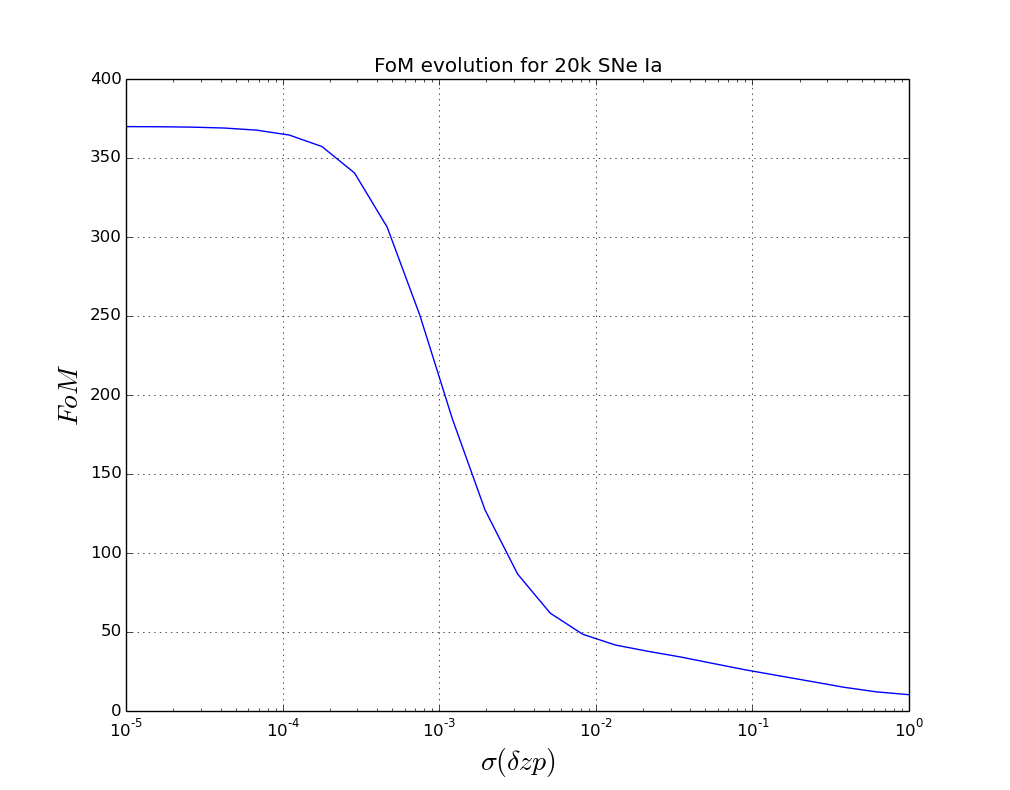
\includegraphics[width=0.7\linewidth]{FoM_20k.png}
  \caption{Evolution of the $FoM$ with the uncertainty on the $\delta zp$'s.}
  \label{fig:fom_zp}
\end{figure}


Expliquer l'algèbre linéaire : Pas de fit --> on calcule seulement la matrice de Fisher \\
Dire que du coup tout se fait assez vite (software performances) \\
On montre le calcul de la FoM \\
On montre les plots d'évolution de la FoM (grille ou 2 plots 1D... à voir!) \\
On peut faire tourner le pipeline sur les données de JLA \\

% ----------------------------------------------------------------------

\section{Discussion}
\label{sec:discussion}

Parler du training


% ----------------------------------------------------------------------

\section{Conclusions}
\label{sec:conclusions}

Here's a summary of what we just reported.

We can draw the following well-organized and neatly-formatted conclusions:
\begin{itemize}
  \item This is important.
  \item We can measure some number with some precision.
  \item This has some implications.
\end{itemize}

Here are some parting thoughts.


% ----------------------------------------------------------------------

\subsection*{Acknowledgments}

Here is where you should add your specific acknowledgments, remembering that some standard thanks will be added via the \code{acknowledgments.tex} and \code{contributions.tex} files.

% 
This is the text imported from \code{acknowledgments.tex}, and will be replaced by some standard LSST DESC boilerplate at some point.
% 


\input{contributions}

%{\it Facilities:} \facility{LSST}

% Include both collaboration papers and external citations:
\bibliography{lsstdesc,main}

\end{document}
% ======================================================================
% 
